\documentclass[10pt]{article}

\usepackage[a4paper,margin=0mm]{geometry}
\usepackage{fontspec}
\usepackage{xeCJK}
\usepackage{graphicx}
\usepackage{xcolor}
\usepackage{tikz}
\usepackage{ragged2e}
\usepackage{microtype}
\usepackage[hidelinks]{hyperref}

\pagestyle{empty}
\setlength{\parindent}{0pt}
\setlength{\fboxsep}{0pt}
\hyphenpenalty=10000
\exhyphenpenalty=10000

\IfFileExists{/System/Library/Fonts/HelveticaNeue.ttc}{
  \setmainfont{HelveticaNeue.ttc}[
    Path=/System/Library/Fonts/,
    FontIndex=0,
    BoldFont=HelveticaNeue.ttc,
    BoldFeatures={FontIndex=1},
    ItalicFont=HelveticaNeue.ttc,
    ItalicFeatures={FontIndex=2},
    BoldItalicFont=HelveticaNeue.ttc,
    BoldItalicFeatures={FontIndex=3}
  ]
}{
  \setmainfont{TeX Gyre Heros}
}

\IfFileExists{/System/Library/Fonts/Optima.ttc}{
  \newfontfamily\displayfont{Optima.ttc}[
    Path=/System/Library/Fonts/,
    FontIndex=0,
    BoldFont=Optima.ttc,
    BoldFeatures={FontIndex=1},
    ItalicFont=Optima.ttc,
    ItalicFeatures={FontIndex=2},
    BoldItalicFont=Optima.ttc,
    BoldItalicFeatures={FontIndex=3}
  ]
}{
  \newfontfamily\displayfont{TeX Gyre Heros}
}

\IfFontExistsTF{PingFang TC}{
  \setCJKmainfont{PingFang TC}[BoldFont={PingFang TC Semibold}]
}{
  \setCJKmainfont{Heiti TC}
}

\definecolor{OrionInk}{HTML}{10283D}
\definecolor{OrionText}{HTML}{334B5C}
\definecolor{OrionMuted}{HTML}{687B88}
\definecolor{OrionBlue}{HTML}{42A7DA}
\definecolor{OrionBlueDark}{HTML}{176B99}
\definecolor{OrionCoral}{HTML}{D46B54}
\definecolor{OrionSage}{HTML}{668B7F}
\definecolor{OrionMist}{HTML}{F3F7F7}
\definecolor{OrionIce}{HTML}{E6F0F3}
\definecolor{OrionLine}{HTML}{D3E0E4}
\definecolor{OrionWhite}{HTML}{FFFFFF}

\newcommand{\place}[4]{%
  \tikz[remember picture,overlay]{%
    \node[anchor=north west,inner sep=0pt,text width=#3] at
    ([xshift=#1,yshift=-#2]current page.north west) {#4};%
  }%
}

\newcommand{\statblock}[3]{%
  \centering
  \makebox[\linewidth][c]{{\displayfont\fontsize{27}{27}\selectfont\bfseries\color{OrionCoral}#1}}\par
  \vspace{0.35mm}
  \parbox[c][4.2mm][c]{\linewidth}{\centering\fontsize{8.8}{9.8}\selectfont\bfseries\color{OrionInk}#2}\par
  \vspace{0.35mm}
  \parbox[t][5mm][t]{\linewidth}{\centering\fontsize{7.5}{9}\selectfont\color{OrionMuted}#3}%
}

\newcommand{\compareicon}{\tikz[baseline=-0.55mm,x=0.65mm,y=0.65mm]{\draw[OrionBlue,line width=0.42mm] (0,1.8)--(3.5,1.8)--(2.6,2.7) (3.5,1.8)--(2.6,0.9);\draw[OrionBlue,line width=0.42mm] (3.5,-0.1)--(0,-0.1)--(0.9,0.8) (0,-0.1)--(0.9,-1);}}
\newcommand{\recordicon}{\tikz[baseline=-0.55mm,x=0.65mm,y=0.65mm]{\draw[OrionBlue,line width=0.42mm] (1.7,0.8) circle (1.7);\draw[OrionBlue,line width=0.42mm] (1.7,0.8)--(1.7,2)--(2.7,0.8);}}
\newcommand{\delivericon}{\tikz[baseline=-0.55mm,x=0.65mm,y=0.65mm]{\draw[OrionBlue,line width=0.42mm] (0,2.5) rectangle (2.8,-1);\draw[OrionBlue,line width=0.42mm] (0.6,1.5)--(2.2,1.5) (0.6,0.7)--(2.2,0.7);\draw[OrionBlue,line width=0.42mm] (3.3,1.8)--(3.3,-0.5) (2.5,0.3)--(3.3,-0.5)--(4.1,0.3);}}

\newcommand{\outputblock}[3]{%
  \centering
  \makebox[\linewidth][c]{#1\hspace{1.5mm}{\fontsize{6.7}{7.5}\selectfont\bfseries\color{OrionBlue}#2}}\par
  \vspace{1mm}
  \makebox[\linewidth][c]{{\displayfont\fontsize{10.8}{11.8}\selectfont\bfseries\color{white}#3}}%
}

\newcommand{\flowblock}[3]{%
  \begin{minipage}[t]{42mm}
    \raggedright
    \parbox[t][4.1mm][t]{42mm}{\displayfont\fontsize{9}{10.2}\selectfont\bfseries\color{OrionCoral}#1}\par
    \vspace{1.1mm}
    \parbox[t][5.3mm][t]{42mm}{\displayfont\fontsize{11.6}{13.2}\selectfont\bfseries\color{OrionInk}#2}\par
    \vspace{1mm}
    \parbox[t][9.2mm][t]{42mm}{\fontsize{8.2}{10.4}\selectfont\color{OrionMuted}#3}
  \end{minipage}%
}

\begin{document}
\begin{tikzpicture}[remember picture,overlay]
  % Quiet product-led canvas with an integrated brand banner.
  \fill[OrionWhite] (current page.south west) rectangle (current page.north east);
  \fill[OrionMist]
    ([yshift=-146mm]current page.north west) rectangle
    ([yshift=-26mm]current page.north east);
  \draw[OrionLine,line width=0.28mm]
    ([xshift=14mm,yshift=-24mm]current page.north west) --
    ([xshift=196mm,yshift=-24mm]current page.north west);
  \fill[OrionCoral]
    ([xshift=14mm,yshift=-23.5mm]current page.north west) rectangle
    ([xshift=45mm,yshift=-24.5mm]current page.north west);

  % Product image, preserved at its native 4:3 ratio.
  \node[anchor=north west,inner sep=0pt] at
    ([xshift=14mm,yshift=-31mm]current page.north west) {
      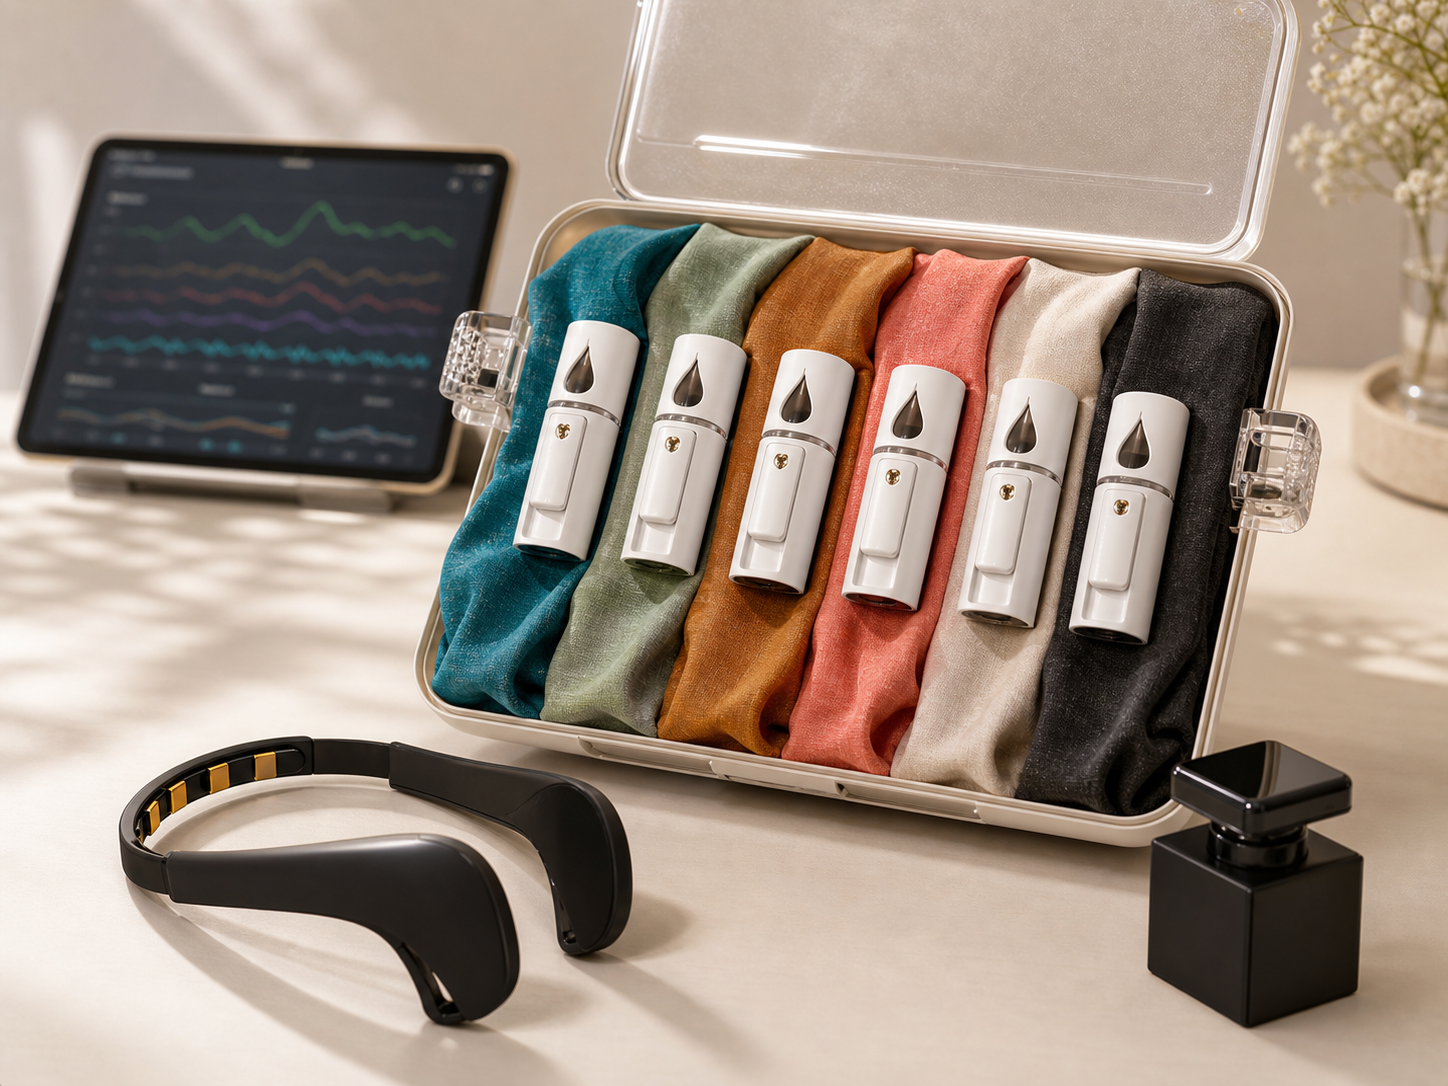
\includegraphics[width=104mm]{../assets/orion-kit.png}
  };
  \draw[OrionLine,line width=0.25mm]
    ([xshift=14mm,yshift=-31mm]current page.north west) rectangle
    ([xshift=118mm,yshift=-109mm]current page.north west);

  % 與主標上緣對齊的珊瑚色標記。
  \fill[OrionCoral]
    ([xshift=124mm,yshift=-33mm]current page.north west) rectangle
    ([xshift=145mm,yshift=-34.1mm]current page.north west);

  % Elevated proof strip with a restrained print-safe shadow.
  \fill[black,opacity=0.055,rounded corners=1.2mm]
    ([xshift=14.8mm,yshift=-114mm]current page.north west) rectangle
    ([xshift=196.8mm,yshift=-141mm]current page.north west);
  \fill[white,rounded corners=1.2mm]
    ([xshift=14mm,yshift=-113mm]current page.north west) rectangle
    ([xshift=196mm,yshift=-140mm]current page.north west);
  \draw[OrionLine,line width=0.22mm]
    ([xshift=73mm,yshift=-117mm]current page.north west) --
    ([xshift=73mm,yshift=-136mm]current page.north west);
  \draw[OrionLine,line width=0.22mm]
    ([xshift=137mm,yshift=-117mm]current page.north west) --
    ([xshift=137mm,yshift=-136mm]current page.north west);

  % Four-step rhythm.
  \foreach \x in {11,61,111,161} {
    \fill[OrionBlue]
      ([xshift=\x mm,yshift=-168mm]current page.north west) rectangle
      ([xshift=\x mm+38mm,yshift=-167.2mm]current page.north west);
  }

  % Muse 去背硬體圖補足流程標題右側的媒體空間。
  \node[anchor=north west,inner sep=0pt] at
    ([xshift=160.5mm,yshift=-149mm]current page.north west) {
      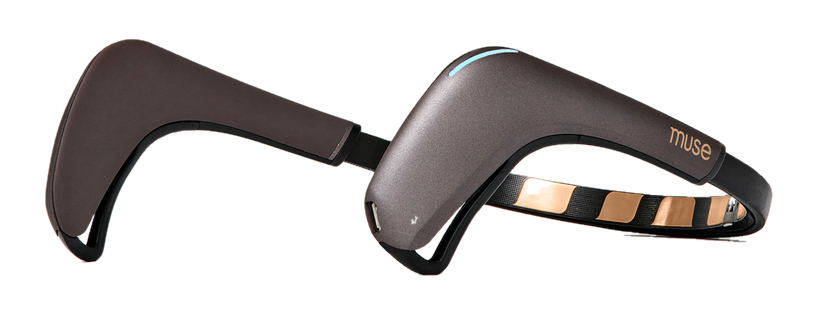
\includegraphics[width=35.5mm]{../assets/muse-device-clean-crop.png}
  };

  % Product interface stage.
  \fill[OrionInk]
    ([yshift=-198mm]current page.north west) rectangle
    (current page.south east);

  % Both Traditional Chinese screenshots stay at their native aspect ratio.
  \node[anchor=north west,inner sep=0pt] at
    ([xshift=14mm,yshift=-216mm]current page.north west) {
      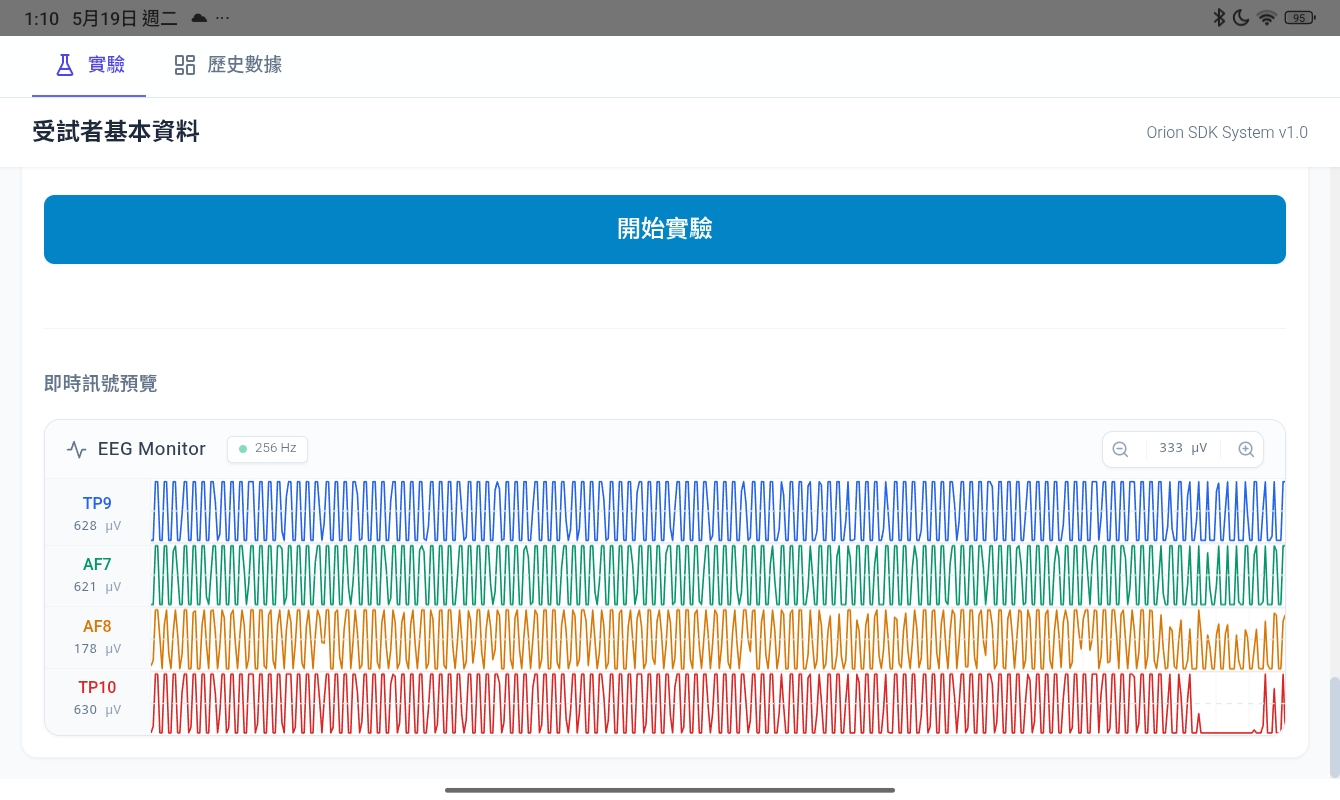
\includegraphics[width=82mm]{../assets/orion-app-screenshot.jpg}
  };
  \node[anchor=north west,inner sep=0pt] at
    ([xshift=114mm,yshift=-216mm]current page.north west) {
      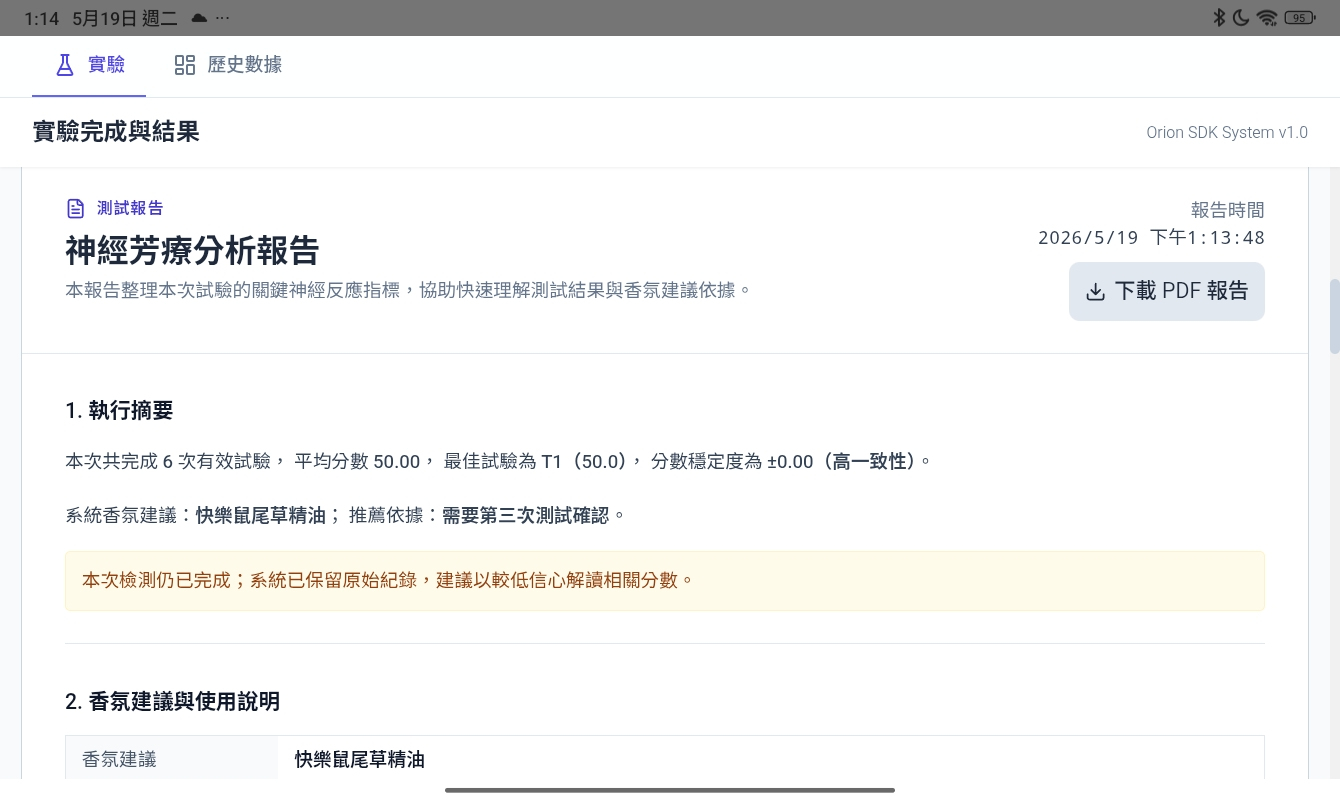
\includegraphics[width=82mm]{../assets/orion-report-screen.jpg}
  };
  \draw[white,opacity=0.34,line width=0.25mm]
    ([xshift=14mm,yshift=-216mm]current page.north west) rectangle
    ([xshift=96mm,yshift=-264.94mm]current page.north west);
  \draw[white,opacity=0.34,line width=0.25mm]
    ([xshift=114mm,yshift=-216mm]current page.north west) rectangle
    ([xshift=196mm,yshift=-264.94mm]current page.north west);

  % 原 Footer 空間改為產品交付內容。
  \draw[white,opacity=0.2,line width=0.25mm]
    ([xshift=14mm,yshift=-271mm]current page.north west) --
    ([xshift=196mm,yshift=-271mm]current page.north west);
  \draw[white,opacity=0.16,line width=0.25mm]
    ([xshift=75mm,yshift=-275mm]current page.north west) --
    ([xshift=75mm,yshift=-292mm]current page.north west);
  \draw[white,opacity=0.16,line width=0.25mm]
    ([xshift=136mm,yshift=-275mm]current page.north west) --
    ([xshift=136mm,yshift=-292mm]current page.north west);
\end{tikzpicture}

% 水平品牌與聯絡頁首。
\place{14mm}{6.1mm}{12mm}{%
  
\includegraphics[width=11mm,height=11mm,keepaspectratio]{orion-ai-app-icon.png}%
}
\place{29mm}{5.2mm}{70mm}{%
  {\displayfont\fontsize{20.5}{21.5}\selectfont\bfseries\color{OrionInk}Orion AI}\par
  \vspace{0.05mm}
  {\fontsize{7.2}{8.2}\selectfont\color{OrionMuted}Petrichor Consulting Co., Ltd.}%
}
\place{103mm}{4.4mm}{67mm}{%
  \raggedleft
  \makebox[67mm][r]{{\fontsize{7.4}{8.4}\selectfont\bfseries\color{OrionBlueDark}\href{https://orion.petrichor.tw/}{orion.petrichor.tw}}}\par
  \vspace{0.45mm}
  \makebox[67mm][r]{{\fontsize{6.5}{7.5}\selectfont\color{OrionMuted}\href{mailto:petrichortpe@gmail.com}{petrichortpe@gmail.com}}}\par
  \vspace{0.45mm}
  \makebox[67mm][r]{{\fontsize{5.8}{6.8}\selectfont\color{OrionMuted}產品、代理與研究合作洽詢}}%
}
\place{176mm}{2.6mm}{20mm}{%
  \centering
  \colorbox{white}{
\includegraphics[width=20mm,height=20mm,keepaspectratio]{orion-ai-line-qr.png}}%
}

% Hero statement.
\place{124mm}{37mm}{72mm}{%
  \raggedright
  {\displayfont\fontsize{23}{30}\selectfont\bfseries\color{OrionInk}
    讓香氣反應，\linebreak 成為可見的證據。}\par
  \vspace{3.2mm}
  {\fontsize{9.8}{15.6}\selectfont\color{OrionText}
    Orion AI 整合 Muse EEG、引導式香氣測試、演算法輔助的 SRI 反應比較與報告交付，形成一套完整研究系統。}\par
  \vspace{2.6mm}
  {\fontsize{8.8}{13.2}\selectfont\bfseries\color{OrionBlueDark}
    在記憶與語言重新詮釋感受之前，捕捉更接近當下的反應訊號。}\par
  \vspace{2.8mm}
  {\fontsize{8.4}{13.2}\selectfont\bfseries\color{OrionInk}
    Muse 頭帶\hspace{1mm}\textbar\hspace{1mm} 六種香氣樣本\par
    Android 測試\hspace{1mm}\textbar\hspace{1mm} 可分享報告}%
}

% Product facts.
\place{18mm}{115.5mm}{51mm}{%
  \statblock{4}{EEG 感測器}{兩個前額、兩個耳側感測點。}%
}
\place{79mm}{115.5mm}{52mm}{%
  \statblock{6}{香氣樣本}{六種引導式樣本，一套比較流程。}%
}
\place{141mm}{115.5mm}{51mm}{%
  \statblock{1}{完整研究紀錄}{SRI、雲端紀錄與 PDF 報告。}%
}

% Workflow.
\place{11mm}{149mm}{142mm}{%
  {\displayfont\fontsize{16.5}{17.5}\selectfont\bfseries\color{OrionInk}
    從基線到報告，一套可重複的測試流程。}\par
  \vspace{1mm}
  {\fontsize{8.4}{10}\selectfont\color{OrionText}
    受試者、香氣、訊號與結果，保留在同一份研究紀錄中。}%
}
\place{11mm}{170.5mm}{188mm}{%
  \flowblock{01 / 基線}{建立參考值}{連接 Muse 並建立受試者個人基線。}
  \hfill
  \flowblock{02 / 測試}{引導香氣測試}{依序執行準備、聞香與休息階段。}
  \hfill
  \flowblock{03 / 比較}{檢視 SRI}{比較 SRI 結果與個人基線的反應變化。}
  \hfill
  \flowblock{04 / 交付}{保留紀錄}{儲存測試並開啟 PDF 結果報告。}%
}

% Real interface proof.
\place{14mm}{202.5mm}{82mm}{%
  {\fontsize{7.8}{8.8}\selectfont\bfseries\color{OrionBlue}即時測試}\par
  \vspace{0.8mm}
  {\displayfont\fontsize{11.8}{12.7}\selectfont\bfseries\color{white}即時 EEG，引導完整測試流程。}\par
  \vspace{0.55mm}
  {\fontsize{7.2}{8.3}\selectfont\color{white!62}四個通道在測試過程中持續顯示。}%
}
\place{114mm}{202.5mm}{82mm}{%
  {\fontsize{7.8}{8.8}\selectfont\bfseries\color{OrionBlue}結果報告}\par
  \vspace{0.8mm}
  {\displayfont\fontsize{11.8}{12.7}\selectfont\bfseries\color{white}完成後，即可交付報告。}\par
  \vspace{0.55mm}
  {\fontsize{7.2}{8.3}\selectfont\color{white!62}測試脈絡、SRI 結果與 PDF 報告完整保留。}%
}

% 交付內容。
\place{14mm}{276mm}{55mm}{%
  \outputblock{\compareicon}{比較}{SRI 與個人基線}%
}
\place{79mm}{276mm}{52mm}{%
  \outputblock{\recordicon}{紀錄}{完整測試歷程}%
}
\place{141mm}{276mm}{55mm}{%
  \outputblock{\delivericon}{交付}{可分享 PDF}%
}
\place{14mm}{293mm}{182mm}{%
  \makebox[182mm][c]{{\fontsize{6.3}{7.2}\selectfont\color{white!58}
    本產品僅供研究與產品評估使用，不作為醫療診斷用途。}}%
}

\end{document}
